\documentclass[border=0pt]{standalone}
\usepackage{tikz,amssymb,url,amsmath,amsthm,listings,algorithm,algpseudocode,enumerate, caption, xspace, float, verbatim,tabularx,mathtools,adjustbox,pgfplots}
\usetikzlibrary{fit}
\usetikzlibrary{positioning}
\usetikzlibrary{math}
\usetikzlibrary{shapes.misc}
\usetikzlibrary{backgrounds}
\def\bw{{\boldsymbol w}}
\def\bx{{\boldsymbol x}}
\def\balpha{{\boldsymbol \alpha}}
\pgfdeclarelayer{background}
\pgfsetlayers{background,main}
\tikzset{cross/.style={cross out, draw=black, minimum size=2*(#1-\pgflinewidth), inner sep=0pt, outer sep=0pt},cross/.default={1pt}}
\begin{document}
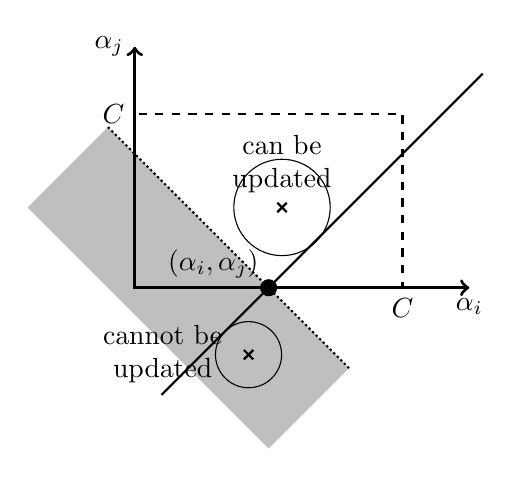
\begin{tikzpicture}[domain=-0.5:4,yscale=1.7,xscale=1.7,baseline,tight background]
	\tikzmath{\lx=0; \ly=0; \ux=2; \uy=1.3; \d=0.5;
	\dl=\lx-\d; \dr=\ux+\d; \da=\uy+\d; \db=\ly-\d;
	\dax=(\lx+\ux)/2; \day=\ly; \dbx=\ux; \dby=-\dax+\day+\dbx;
	\dda=0.8; \daax=\dax-\dda; \daay=\day-\dda; 
	\ddb=0.6; \dbax=\dbx+\ddb; \dbay=\dby+\ddb;
	\dab=1.2; \dabx=\dax-\dab; \daby=\day+\dab; 
	\dbb=0.6; \dbbx=\dax+\dbb; \dbby=\day-\dbb;
	\dac=1.2; \dacx=\dabx-0.6; \dacy=\daby-0.6; 
	\dbc=0.6; \dbcx=\dbbx-0.6; \dbcy=\dbby-0.6;
	\cax=0.85; \cay=-0.5; \ra=0.247;
	\cbx=1.1; \cby=0.6; \rb=0.36;
	\caplx=0.35*\lx+0.65*\ux; \caply=\da;
	}
	\draw[-, dashed, thick] (\lx,\ly) -- (\ux,\ly) node[below]{$C$} -- (\ux,\uy) -- (\lx,\uy) node[left]{$C$} -- (\lx,\ly);
	\filldraw[black] (\dax,\day) node[above]{$(\alpha_i,\alpha_j)\qquad\quad\quad$} circle (1.7pt);
	\draw[<->, very thick] (\lx,\da) node[left]{$\alpha_j$} -- (\lx,\ly) -- (\dr,\ly) node[below]{$\alpha_i$};
	\draw[-, thick] (\daax, \daay) -- (\dbax, \dbay);
	\draw[black] (\cax, \cay) node[left]{\begin{tabular}{c} cannot be\\ updated\end{tabular}} circle (\ra);
	\draw (\cax, \cay) node[cross=2.5pt,thick]{};
	\draw[black] (\cbx, \cby) node[above]{\begin{tabular}{c} can be\\ updated\end{tabular}} circle (\rb);
	\draw (\cbx, \cby) node[cross=2.5pt,thick]{};
	\draw[-, densely dotted, thick] (\dabx, \daby) -- (\dbbx, \dbby);
	\begin{pgfonlayer}{background}
		\fill[lightgray] (\dabx, \daby) to (\dbbx, \dbby) to (\dbcx, \dbcy) to (\dacx, \dacy) to (\dabx, \daby);
	\end{pgfonlayer}
	%\node at (\caplx, \caply){With a Linear Constraint};
\end{tikzpicture}
\end{document}
